%%%%%%%%%%%%%%%%%%%%%%%%%%%%%%%%%
%
%このファイルは3回のコンパイルの後,
%同梱の./listofcontents.shを用いて
%./listofcontents.sh ファイル名からドットと拡張子を除いたもの
%を1回実行し,最後にもう一度コンパイルをする必要があります.
%
%また,同梱のkanzawa.sty, kanzawa_m.sty, kanzawa2.sty, moreverb.*,
%listofcontents.sh, here.sty, jtygm.sty,
%も必要になります.
%
%
%%%%%%%%%%%%%%%%%%%%%%%%%%%%%%%%%%%
\documentclass[a4j,12pt,dvipdfmx,oneside]{jsbook}

\usepackage[subrefformat=parens]{subcaption}
\usepackage{kanzawa2}
\usepackage{here}
\usepackage{times}
\usepackage{amsmath,amsthm,amssymb}
\theoremstyle{definition}
\newtheorem{theorem}{定理}
\newtheorem*{theorem*}{定理}
\newtheorem{Def}[theorem]{定義}
\newtheorem*{Def*}{定義}
\newtheorem{Alg}[theorem]{アルゴリズム}
\newtheorem*{Alg*}{アルゴリズム}
\usepackage{mathptmx}
\usepackage{pifont}
\usepackage{tascmac}
\usepackage{oldgerm}
\usepackage{jtygm}
\usepackage{type1cm}
\setlength{\textwidth}{\fullwidth}
\newcommand{\vd}{\mbox{d}}
\def\rthree{I\kern-2ptI\kern-2ptI}
\newcommand{\namelistlabel}[1]{\mbox{#1}\hfil}
\newenvironment{namelist}[1]{
\begin{list}{}
 {\let\makelabel\namelistlabel
 \settowidth{\labelwidth}{#1}
 \setlength{\leftmargin}{1.1\labelwidth}}
 }{
\end{list}}

\usepackage[T1]{fontenc}
\usepackage{textcomp}
\usepackage[utf8]{inputenc}
\usepackage{lmodern}
\usepackage[all, warning]{onlyamsmath}
\kanjiencoding{JY1}
\kanjifamily{mc}
\kanjiseries{m}
\kanjishape{n}
\selectfont
\usepackage{enumitem}
\newcommand{\argmax}{\operatornamewithlimits{\mathrm{arg\,max}}}
\newcommand{\argmin}{\operatornamewithlimits{\mathrm{arg\,min}}}
\newcommand{\QED}{\hfill$\blacksquare$\par}
\usepackage{longtable}
\usepackage[dvipdfmx]{graphicx}
\usepackage{mediabb}
\makeatletter
\def\minimize{\mathop{\operator@font minimize}} 
\makeatother
\usepackage{eclbkbox}	% required for `\breakbox' (yatex added)
\begin{document}
\pagestyle{headings}
\def\thepage{\roman{page}}
\input epsf
\tableofcontents
\listoffigures
\listoftables
%%%%%
\newpage
\pagestyle{myheadings}

\chapter{序論}
\def\thepage{\arabic{page}}
\setcounter{page}{1}
\label{chap:first}

 \section{背景}\label{sec:background}
 
 近年,情報通信社会の発展に伴いデータ量が増大し,日々多様なデータがコンピュータに蓄積されている.
 検索エンジンなどのインターネット上のサービスでは,蓄積されたビッグデータの解析や分類を行うことで,
 利用者に適切な情報を素早く送ることを可能にしている.
 ビッグデータを人の手によって分類することには困難が伴うため,
 計算機を用いて自動的にデータの分類を行うための技術であるクラスタリングが必要となる.
 クラスタリングとは,与えられたデータの個体間に存在する類似性に基づいて,
 個体をいくつかのクラスタと呼ばれるグループに分割を行う教師なし機械学習の手法である.
 図~\ref{fig:about_clustering}に示すように,ある一定のルールに従って存在するデータがあったときに,
 クラスタリングを行うことでそれぞれのデータがどのクラスタに属するかということを示すことができる.
 
 データをクラスタに分類した際に,それぞれのデータが各クラスタに属す度合いを表した値を帰属度と呼ぶ.
 帰属度が0と1のみで表され,
 それぞれのデータが各クラスタに明確に分類されるクラスタリングをハードクラスタリングと呼び,
 一方で帰属度が0と1の間の値で表され,
 データが属するクラスタを柔軟に表すことができるクラスタリングをファジィクラスタリングと呼ぶ.
 現実に存在しているデータには,明確に分類できるものだけでなく本質的に分類できない複雑なものも存在し,
 そういったデータの分類にはファジィクラスタリングが有効である.

 \begin{figure}[htbp]
  \centering
  \begin{minipage}{0.4\hsize}
   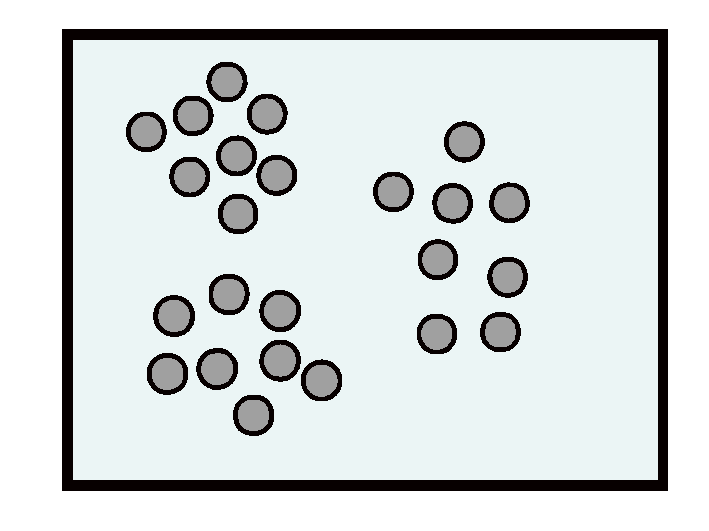
\includegraphics[width=\linewidth]{before_clustering.pdf}
   \subcaption{クラスタリング前}
  \end{minipage}
  \begin{minipage}{0.4\hsize}
   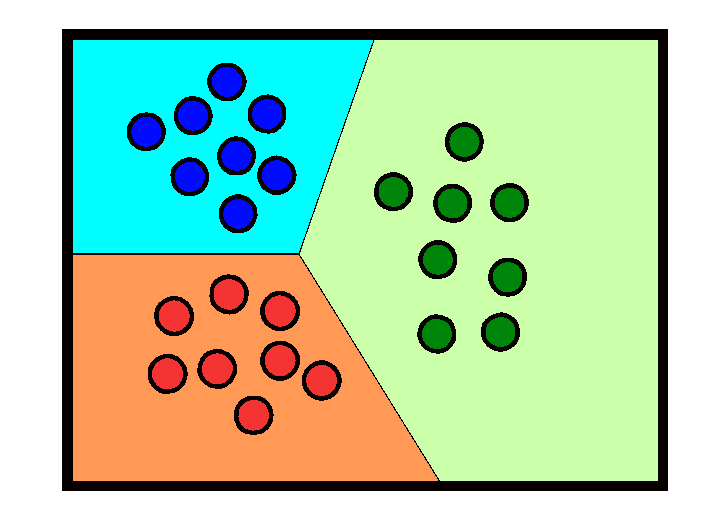
\includegraphics[width=\linewidth]{after_clustering.pdf}
   \subcaption{クラスタリング後}
  \end{minipage}
  \caption{クラスタリングについて}
  \label{fig:about_clustering}
 \end{figure}

 \newpage
 
 \section{目的}\label{sec:purpose}

 既存の手法における課題として,各クラスタのサイズに差がある場合,
 クラスタリングから有意な結果が得られないというものがある.
 ここで,クラスタのサイズとは,クラスタに属するデータの数と,そのクラスタに属するデータ間の類似度に基づくものであり,
 データの数が多い,または類似度が小さいクラスタをサイズが大きいクラスタとし,
 データの数が少ない,または類似度が大きいクラスタをサイズが大きいクラスタとする.
 現在,各クラスタのサイズを考慮してクラスタリングを行う手法が複数提案されており,
 本研究はその中でも,
 Standard Fuzzy $c$-Means with vAriable controlling cluster size~(sFCMA)~\cite{sFCMA},
 Entropy-regularized Fuzzy $c$-Means vAriable controlling clusters size~(eFCMA)~\cite{eFCMA},
 $q$-divergence based Fuzzy $c$-Means with vAriable controlling cluster size~(qFCMA)~\cite{qFCMA}
 の$3$手法について,各手法の特性を把握するとともに,最も有効な手法を発見することを目的とする.

 \section{構成}\label{sec:contents}
 本文書の構成を次に示す.
 第\ref{chap:suggest_method}章では,提案手法について説明する.
 第\ref{chap:artificial_data}章では,人工データ実験による各手法の特性比較を行う.
 第\ref{chap:real_data}章では,実データ実験による各手法の精度比較を行う.
 最後に第\ref{chap:conclusion}章では,本文書の結論を述べる.
 また,付録では,プログラムソースを掲載している.

\chapter{提案手法}\label{chap:suggest_method}

 \section{はじめに}\label{sec:suggest_method_intro}
 本章では,本研究で提案するファジィクラスタリング手法について説明する.
 まず第~\ref{sec:suggest_method_define}節で定義を示し,
 次に第~\ref{sec:efcma}節から第~\ref{sec:qfcma}節で各手法の最適化問題と,各変数の更新式について述べる.
 
 \section{定義}\label{sec:suggest_method_define}
 
 次節で述べるファジィクラスリングの最適化問題における各変数の定義について,表~\ref{tab:fuzzy_c_define}に示す.
 \begin{table}[htbp]
  \caption{ファジイクラスタリングの最適化問題における定義}
  \begin{center}
   \begin{tabular}{c|c||c|c} \hline
    {$N$}&データ数&{$x_k$}&データ \\ \hline
    {$C$}&クラスタ数&{$v_i$}&クラスタ中心\\ \hline
    {$\lambda$,~$m$}&ファジィ化パラメータ&{$u_{i,k}$}&帰属度 \\ \hline
    {$\alpha_i$}&クラスタサイズ調整変数\\ \hline
   \end{tabular}
  \end{center}
  \label{tab:fuzzy_c_define}
 \end{table}

 \section{sFCMA}\label{sec:sfcma}
 
 Standard Fuzzy $c$-Means with vAriable controlling cluster size~(sFCMA)~\cite{sFCMA}
 の最適化問題を以下に示す.
 \begin{align}
  &\underset{u,v,\alpha}{\text{minimize}}
  \sum_{i=1}^C\sum_{k=1}^N(\alpha_{i})^{1-m}(u_{i,k})^m||x_k-v_i||_2^2\\
  &{\text{subject to }}\sum_{i=1}^Cu_{i,k}=1,~\sum_{i=1}^C\alpha_{i}=1{\text{ and }}m>1,~\alpha_{i}>0
 \end{align}
 次に,クラスタ中心$v_{i}$の更新式を以下に示す.
 \begin{align}
  v_{i}=\frac{\sum_{k=1}^N(u_{i,k})^mx_{k}}{\quad\sum_{k=1}^N(u_{i,k})^{m}}
 \end{align}
 次に,帰属度$u_{i,k}$の更新式を以下に示す.
 \begin{align}
  u_{i,k}=\frac{1}{\sum_{j=1}^c\frac{\alpha_{j}}{\alpha_{i}}\left(\frac{d_{j,k}}{d_{i,k}}\right)^\frac{1}{1-m}}
 \end{align}
 次に,クラスタサイズ調整変数$\alpha_{i}$の更新式を以下に示す.
 \begin{align}
  \alpha_{i}=\frac{1}{\sum_{j=1}^C\left(\sum_{k=1}^N\frac{(u_{j,k})^md_{j,k}}{(u_{i,k})^md_{i,k}}\right)^{\frac{1}{m}}}
 \end{align}

 \section{eFCMA}\label{sec:efcma}

 Entropy-regularized Fuzzy $c$-Means vAriable controlling clusters size~(eFCMA)~\cite{eFCMA}
 の最適化問題を以下に示す.
 \begin{align}
  \underset{u,v,\alpha}{\text{minimize}}
  \sum_{i=1}^C\sum_{k=1}^Nu_{i,k}||x_k-v_i||_2^2+\lambda^{-1}\sum_{i=1}^C\sum_{k=1}^Nu_{i,k}\log\Bigl(\frac{u_{i,k}}{\alpha_{i}}\Bigl)\\
  {\text{subject to }}\sum_{i=1}^Cu_{i,k}=1,~\sum_{i=1}^C\alpha_{i}=1{\text{ and }}\lambda>0,~\quad\alpha_{i}>0
 \end{align}
 次に,クラスタ中心$v_{i}$の更新式を以下に示す.
 \begin{align}
  v_{i}=\frac{\sum_{k=1}^Nu_{i,k}x_{k}}{\quad\sum_{k=1}^Nu_{i,k}}
 \end{align}
 次に,帰属度$u_{i,k}$の更新式を以下に示す.
 \begin{align}
  u_{i,k}=\frac{\alpha_{i}\exp(-\lambda||x_k-v_i||_2^2)}{\sum_{j=1}^C\alpha_{j}\exp(-\lambda||x_k-v_j||_2^2)}
 \end{align}
 次に,クラスタサイズ調整変数$\alpha_{i}$の更新式を以下に示す.
 \begin{align}
  \alpha_{i}=\frac{\sum_{k=1}^Nu_{i,k}}{\quad N}
 \end{align}

 \section{qFCMA}\label{sec:qfcma}
 
 $q$-divergence based Fuzzy $c$-Means with vAriable controlling cluster size~(qFCMA)~\cite{qFCMA}
 の最適化問題を以下に示す.
 \begin{align}
  \underset{u,v,\alpha}{\text{minimize}}
  \sum_{i=1}^C\sum_{k=1}^N(\alpha_{i})^{1-m}(u_{i,k})^m||x_k-v_i||_2^2
  +\frac{\lambda^{-1}}{m-1}\sum_{i=1}^C\sum_{k=1}^N(\alpha_{i})^{1-m}(u_{i,k})^m\\
  {\text{subject to }}\sum_{i=1}^Cu_{i,k}=1,~\sum_{i=1}^C\alpha_{i}=1{\text{ and }}\lambda>0,~m>1,~\alpha_{i}>0
 \end{align}
 次に,クラスタ中心$v_{i}$の更新式を以下に示す.
 \begin{align}
  v_{i}=\frac{\sum_{k=1}^N(u_{i,k})^mx_{k}}{\quad\sum_{k=1}^N(u_{i,k})^{m}}
 \end{align}
 次に,帰属度$u_{i,k}$の更新式を以下に示す.
 \begin{align}
  u_{i,k}=\frac{\alpha_{i}(1+\lambda(1-m)||x_i-v_k||_2^2)^\frac{1}{1-m}}{\quad\sum_{j=1}^C\alpha_{j}(1+\lambda(1-m)||x_j-v_k||_2^2)^\frac{1}{1-m}}
 \end{align}
 次に,クラスタサイズ調整変数$\alpha_{i}$の更新式を以下に示す.
 \begin{align}
  \alpha_{i}=\frac{1}{\sum_{j=1}^C\left(\sum_{k=1}^N\frac{(u_{j,k})^m(1-\lambda(1-m)d_{j,k})}{(u_i,k)^m(1-\lambda(1-m)d_{i,k})}\right)^{\frac{1}{m}}}
 \end{align}

 \section{おわりに}\label{sec:suggest_method_summary}
 本章では,本研究で提案するファジィクラスタリング手法について説明した.
 まず第~\ref{sec:suggest_method_define}節で定義を示し,
 次に第~\ref{sec:efcma}節から~\ref{sec:qfcma}節で各手法の最適化問題と,各変数の更新式について述べた.
 
 
 
\chapter{人工データによる実験}\label{chap:artificial_data}

 \section{はじめに}\label{sec:artificial_data_intro}
 本章では,人工データを用いた実験について述べる.
 まず第\ref{sec:about_artificial_data}節で本実験で用いる人工データについて説明する.
 次に第~\ref{sec:artificial_data_algorythm}節でアルゴリズムについて述べる.
 最後に第\ref{sec:classification_function}節で実験により得られた分類関数を用いて各手法の特性比較を行う.
 
 \section{人工データについて}\label{sec:about_artificial_data}
 人工データとして,
 クラス数2,各クラスのデータ数50,合計データ数100のデータを
 平均値($-1$, $-1$),標準偏差($0.5$, $0.5$)
 及び平均値($1$, $1$),標準偏差($0.5$, $0.5$)
 のガウスサンプリングで生成したデータを用いた(図~\ref{fig:artificial_data}).
 \begin{figure}[p]
  \centering
  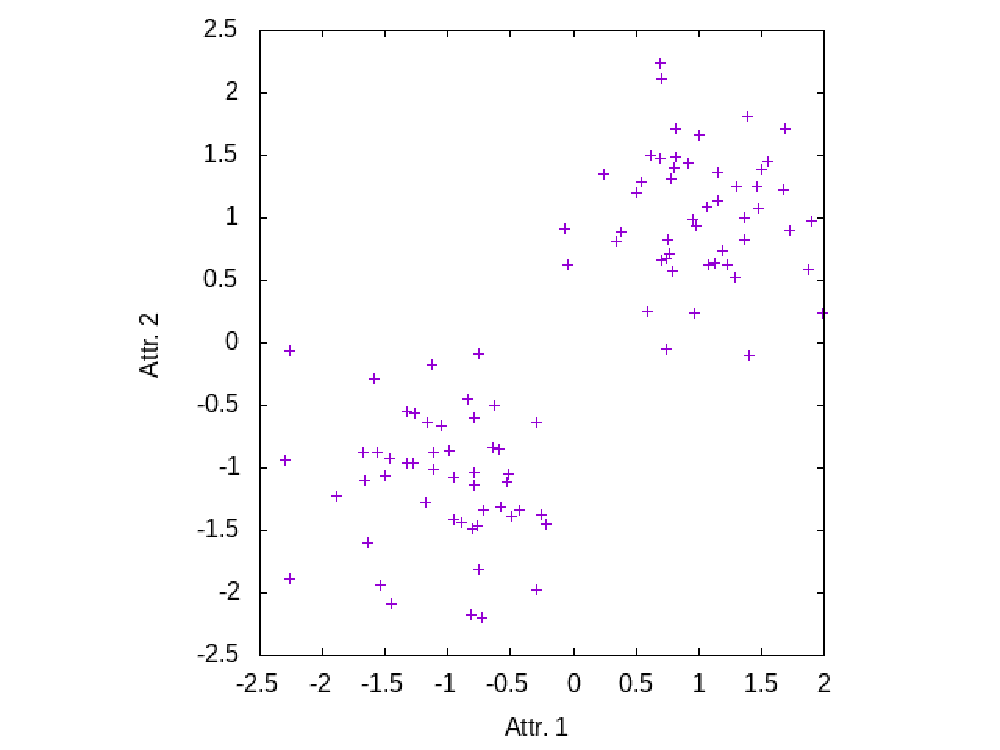
\includegraphics[width=\linewidth]{2d-dat.pdf}
  \caption{人工データ}
  \label{fig:artificial_data}
 \end{figure}

 \section{アルゴリズム}\label{sec:artificial_data_algorythm}
  \begin{enumerate}
   \item 帰属度$u$を正解帰属度で初期化し,クラスタサイズ調整変数$\alpha$をクラスタ数の逆数で初期化する.
   \item 帰属度$u$を用いてクラスタ中心$v$及びクラスタサイズ調整変数$\alpha$を更新する.
   \item $u, v, \alpha$の変化の合計が$10^{-10}$未満に収束すれば終了し,そうでない場合は$2$に戻る.
  \end{enumerate}

  \section{分類関数による特性比較}\label{sec:classification_function}

  分類関数は,各クラスタに対する帰属度を座標空間上に可視化したもので,分類関数を見ることにより,
  データがどのクラスタに属するかということが調べることができるとともに,
  各手法がファジィであるかクリスプであるかを判別することができる.
  
  sFCMAの実験結果を図~\ref{fig:sFCMA-Em2},~\ref{fig:sFCMA-Em11}に示す.
  パラメータ$m$を$2.00$から$1.01$に変化させたところ,分類関数は$m$の値が大きいほどファジィになり,
  小さいほどクリスプになることが分かった.

  \begin{figure}[p]
   \centering
   \begin{minipage}{0.43\hsize}
    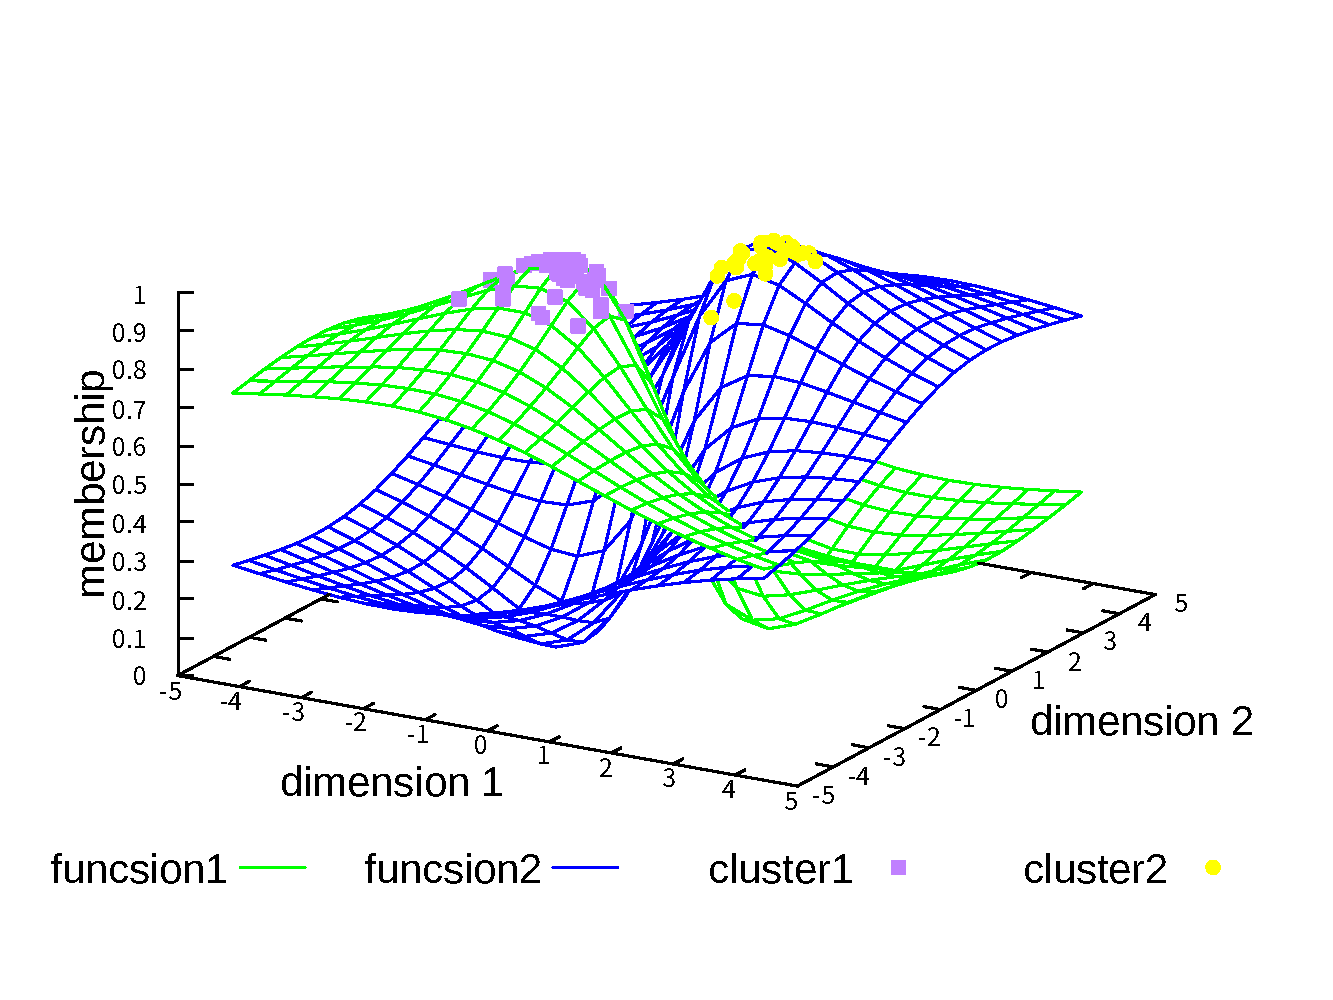
\includegraphics[width=\linewidth]{sFCMA-Em2.pdf}
    \subcaption{$m$=$2.00$}
    \label{fig:sFCMA-Em2}
   \end{minipage}
   \begin{minipage}{0.43\hsize}
    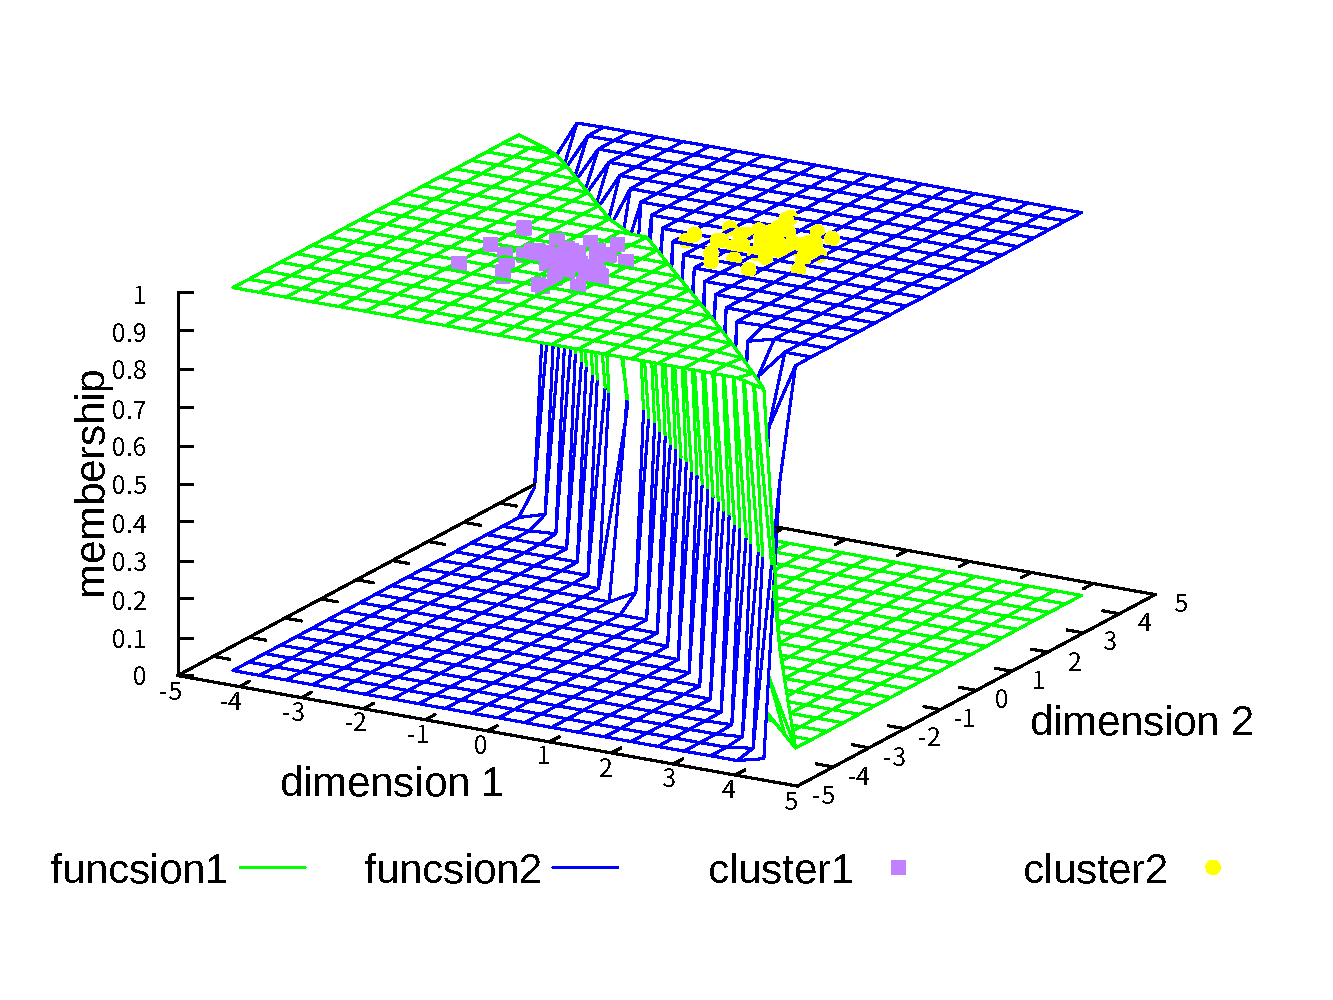
\includegraphics[width=\linewidth]{sFCMA-Em11.pdf}
    \subcaption{$m$=$1.01$}
    \label{fig:sFCMA-Em11}
   \end{minipage}
   \vspace*{0.5cm}
   \caption{sFCMAの人工データの実験結果}
   \label{fig:sFCMA}
  \end{figure}
    
  次に,eFCMAの実験結果を図~\ref{fig:eFCMA-Lambda1},~\ref{fig:eFCMA-Lambda10}に示す.
  垂直軸は分類関数値を,底面はデータ空間を表す.
  網掛けで示されるのが分類関数であり,各点がデータを表している.
  パラメータ$\lambda$を$1$から$10$に変化させたところ,分類関数は$\lambda$の値が小さいほどファジィになり,
  大きいほどクリスプになることが分かった.

  \begin{figure}[p]
   \centering
   \begin{minipage}{0.43\hsize}
    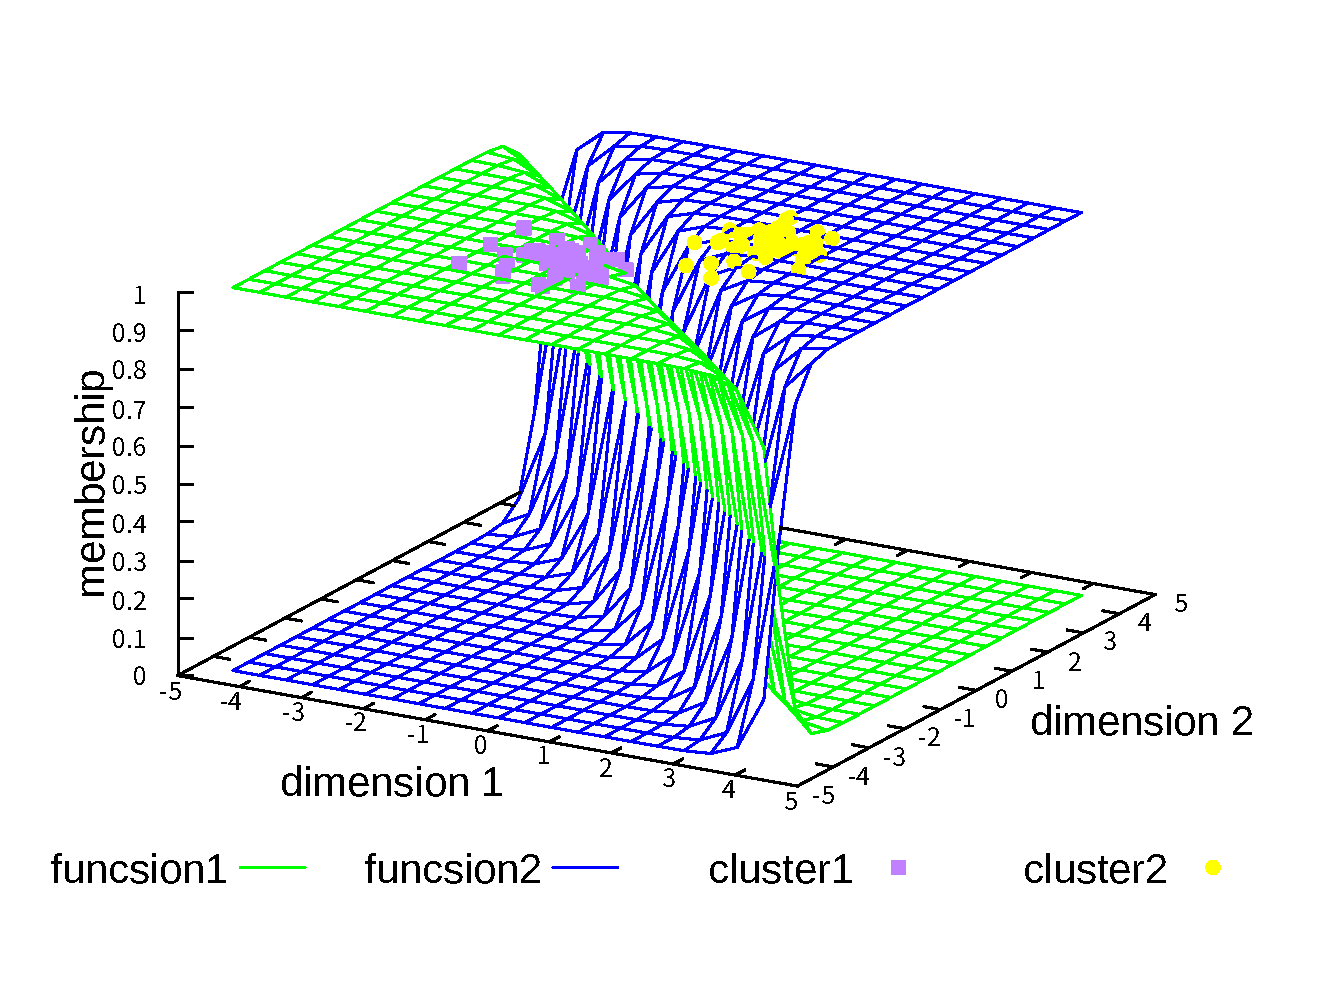
\includegraphics[width=\linewidth]{eFCMA-Lambda1.pdf}
    \subcaption{$\lambda$=$1$}
    \label{fig:eFCMA-Lambda1}
   \end{minipage}
   \begin{minipage}{0.43\hsize}
    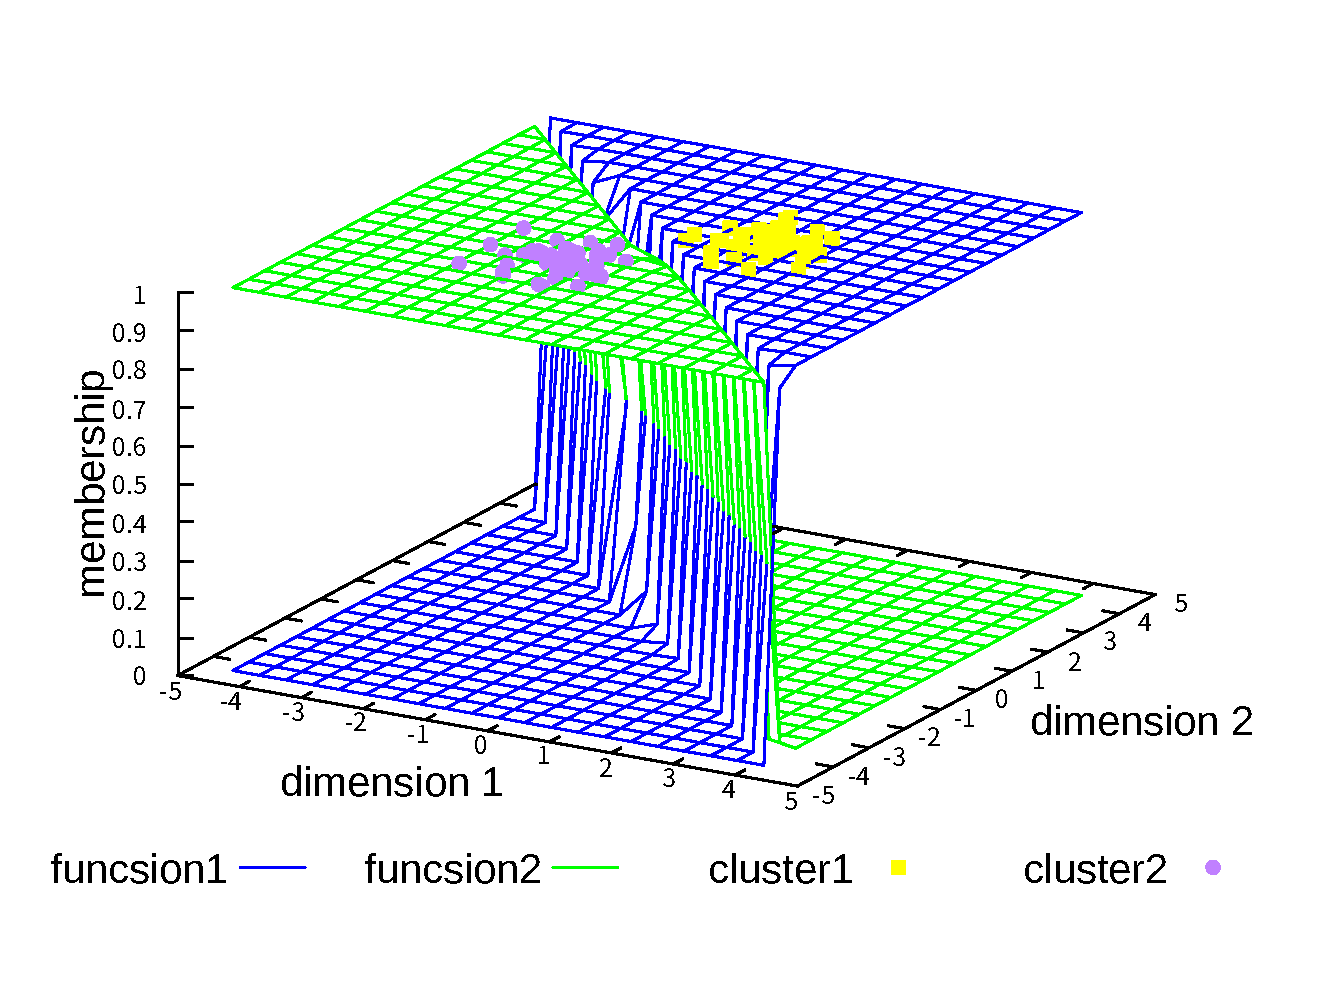
\includegraphics[width=\linewidth]{eFCMA-Lambda10.pdf}
    \subcaption{$\lambda$=$10$}
    \label{fig:eFCMA-Lambda10}
   \end{minipage}
   \vspace*{0.5cm}
   \caption{eFCMAの人工データの実験結果}
   \label{fig:eFCMA}
  \end{figure}
  
  qFCMAの実験結果を
  図~\ref{fig:qFCMA-Em2-Lambda1},~\ref{fig:qFCMA-Em11-Lambda1},~\ref{fig:qFCMA-Em11-Lambda10}
  に示す.
  こちらは,パラメータ($m$, $\lambda$)の組み合わせとして,
  $(2.00, 1)$, $(1.01, 1)$, $(1.01, 10)$
  の3通りでクラスタリングを行った.
  図~\ref{fig:qFCMA-Em2-Lambda1}及び図~\ref{fig:qFCMA-Em11-Lambda1}の分類関数より,
  $m$の値が大きいほどファジィになり,小さいほどクリスプになることが分かった.
  また,図~\ref{fig:qFCMA-Em11-Lambda1}及び図~\ref{fig:qFCMA-Em11-Lambda10}の分類関数より,
  $\lambda$の値が小さいほどファジィになり,大きいほどクリスプになることが分かった.
  そして,図~\ref{fig:sFCMA}及び図~\ref{fig:qFCMA-Em2-Lambda1},~\ref{fig:qFCMA-Em11-Lambda1}
  の分類関数よりqFCMAにおいて$m-1\rightarrow+0$とするとsFCMAと同じ特性が得られ,
  図~\ref{fig:eFCMA}及び図~\ref{fig:qFCMA-Em11-Lambda1},~\ref{fig:qFCMA-Em11-Lambda10}より,
  $\lambda\rightarrow\infty$とするとeFCMAと同様の特性を示すことがわかった.
  これらの実験結果よりqFCMAはsFCMAとeFCMAの特性を併せ持つと言える.

  \begin{figure}[p]
   \centering
   \begin{minipage}{0.43\hsize}
    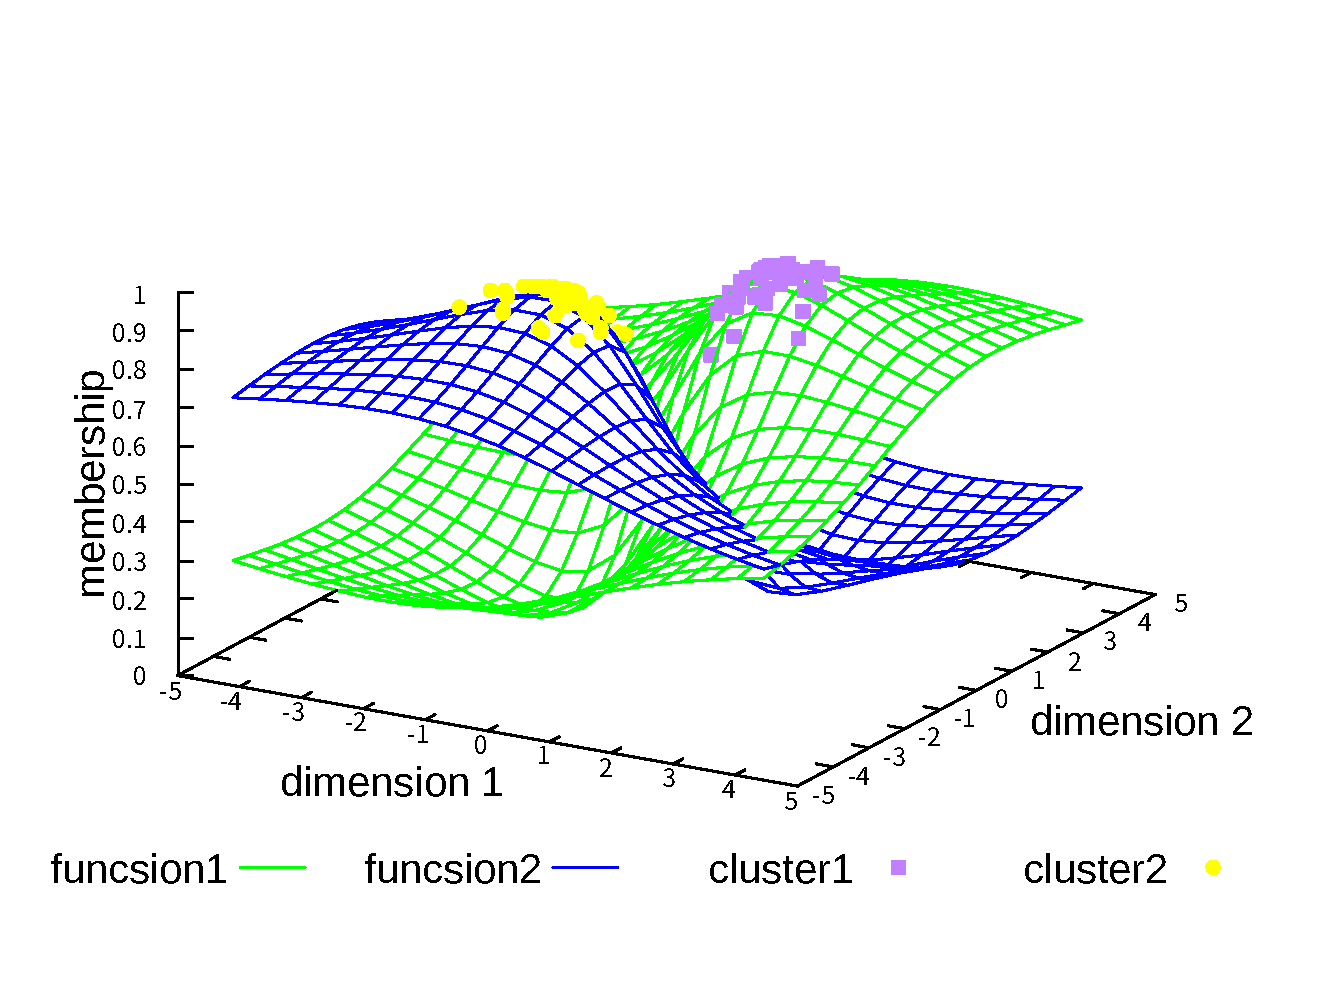
\includegraphics[width=\linewidth]{qFCMA-Em2-Lambda1.pdf}
    \subcaption{$m=2.00$, $\lambda=1$}
    \label{fig:qFCMA-Em2-Lambda1}
   \end{minipage}
   \begin{minipage}{0.43\hsize}
    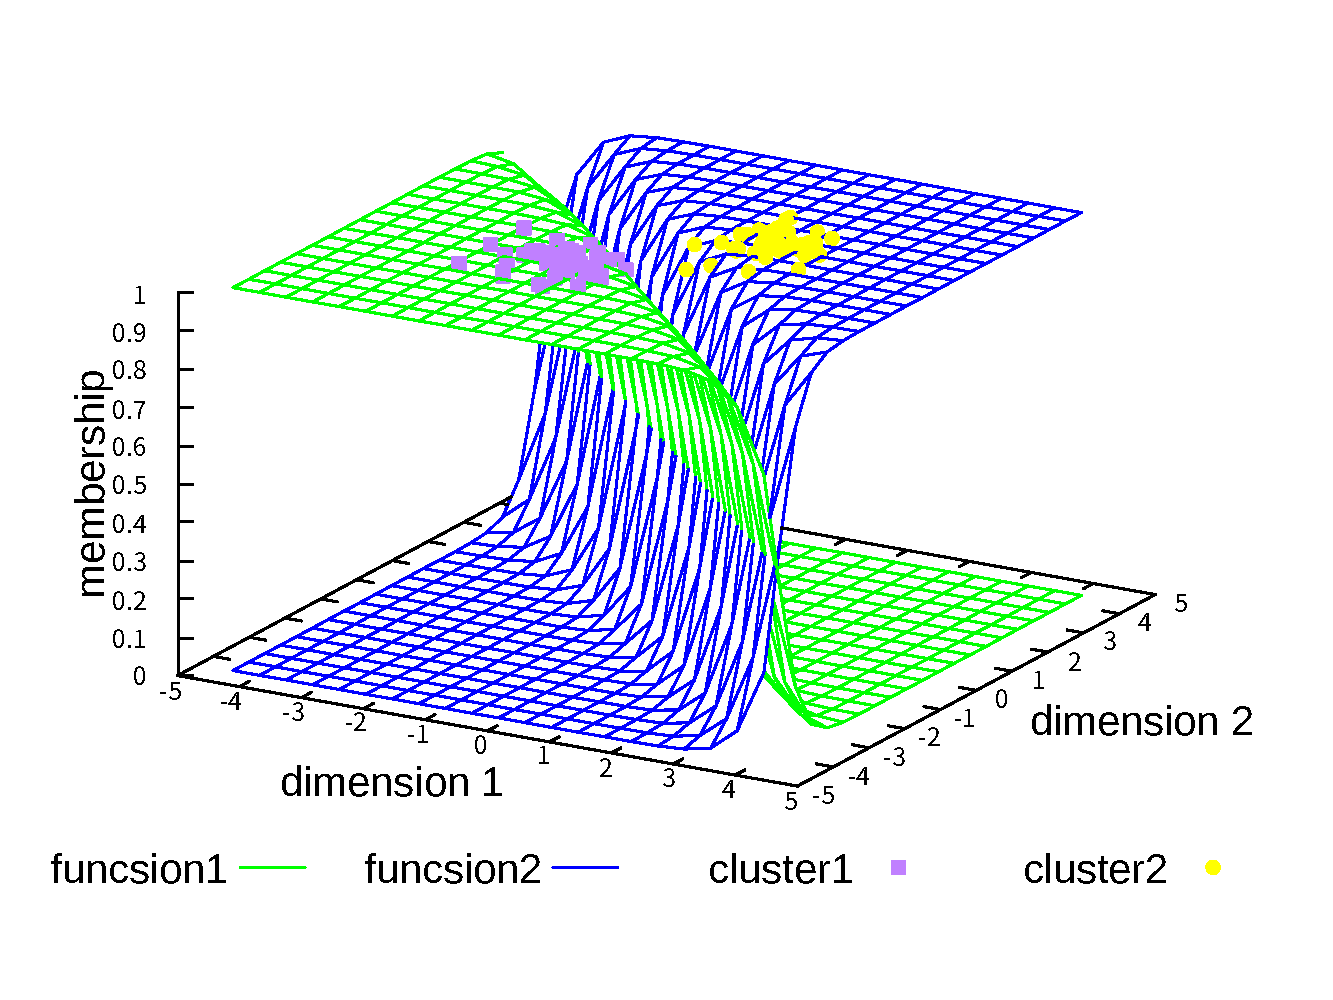
\includegraphics[width=\linewidth]{qFCMA-Em11-Lambda1.pdf}
    \subcaption{$m=1.01$, $\lambda=1$}
    \label{fig:qFCMA-Em11-Lambda1}
   \end{minipage}
   \begin{minipage}{0.43\hsize}
    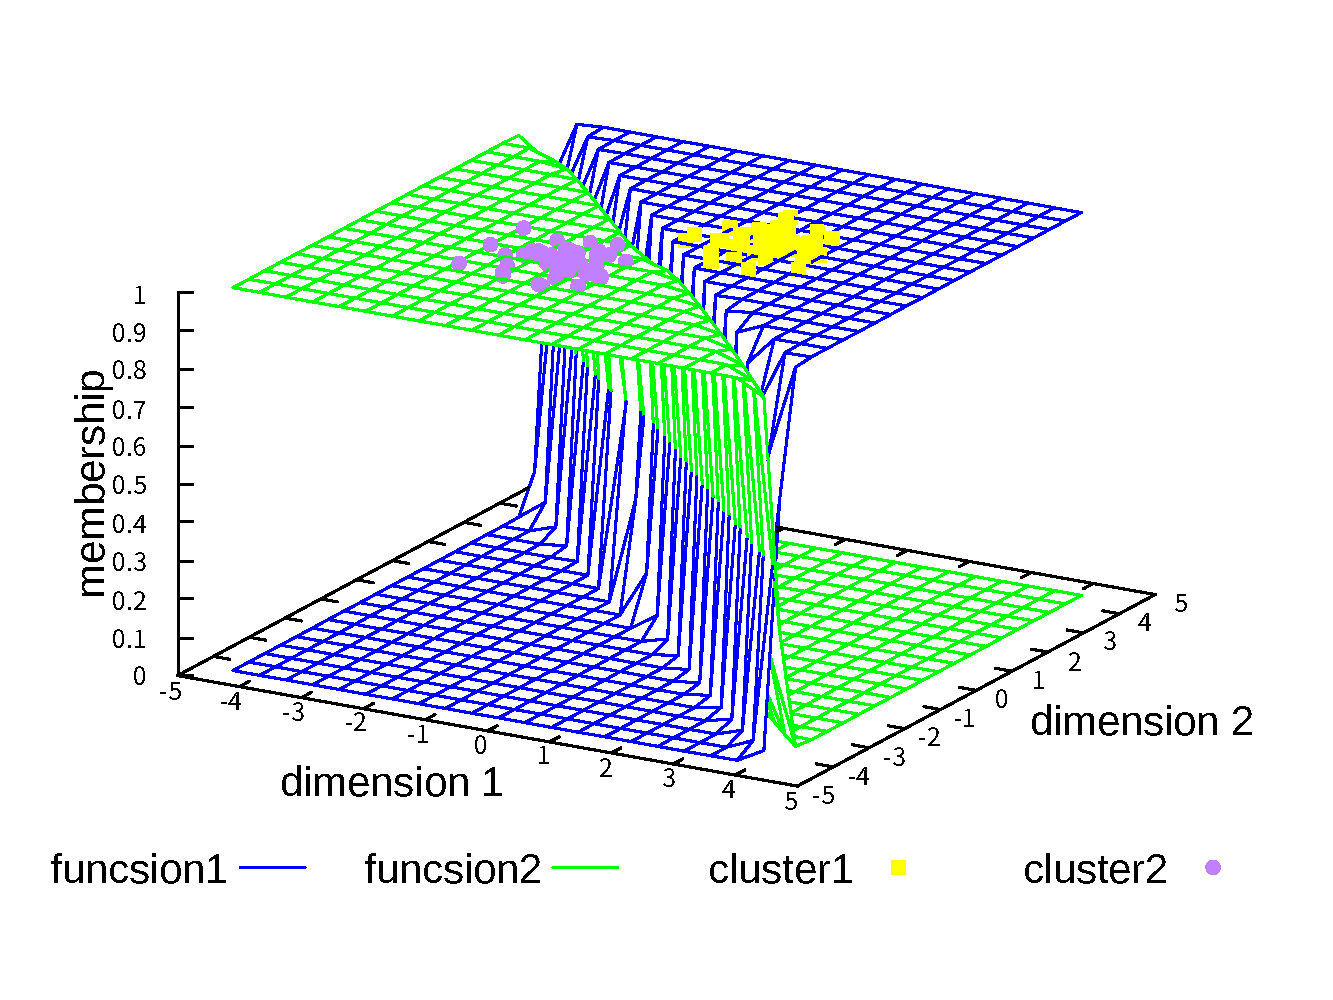
\includegraphics[width=\linewidth]{qFCMA-Em11-Lambda10.pdf}
    \subcaption{$m=1.01$, $\lambda=10$}
    \label{fig:qFCMA-Em11-Lambda10}
   \end{minipage}
   \vspace*{0.5cm}
   \caption{qFCMAの人工データの実験結果}
   \label{fig:qFCMA}
  \end{figure}
  
  \section{おわりに}\label{sec:artificial_data_summary}
  本章では,人工データを用いた実験について述べた.
  まず第\ref{sec:about_artificial_data}節で本実験で用いる人工データについて説明した.
  次に第~\ref{sec:artificial_data_algorythm}節でアルゴリズムについて述べた.
  最後に第\ref{sec:classification_function}節で実験により得られた分類関数を用いて各手法の特性比較を行った.
  
  
\chapter{実データによる実験}\label{chap:real_data}

 \section{はじめに}\label{sec:real_data_intro}
 本章では,実データを用いた実験について述べる.
 まず第\ref{sec:about_real_data}節で本実験で用いる実データについて説明する.
 次に第~\ref{sec:real_data_algorythm}節でアルゴリズムについて述べる.
 最後に第\ref{sec:ari_compare}節で実験により得られた評価指標を用いて各手法の精度比較を行う.
 
 \section{実データについて}\label{sec:about_real_data}
 実データとしては,
 個体数403,
 クラス数4の,
 被験者の勉強時間や試験結果などの5属性を収録した
 ``User Knowledge Modeling Dasta Set''
 を用いた.
 
 \section{アルゴリズム}\label{sec:real_data_algorythm} 
  \begin{enumerate}
   \item 帰属度$u$を正解帰属度で初期化し,クラスタサイズ調整変数$\alpha$をクラスタ数の逆数で初期化する.
   \item 帰属度$u$を用いてクラスタ中心$v$及びクラスタサイズ調整変数$\alpha$を更新する.
   \item $u, v, \alpha$の変化の合計が$10^{-10}$未満に収束すれば終了し,そうでない場合は$2$に戻る.
  \end{enumerate}
  
 \section{ARIによる精度比較}\label{sec:ari_compare}

  sFCMA, eFCMA, qFCMAの実データ実験の結果について,
  それぞれ図~\ref{fig:sFCMA_ARI},~\ref{fig:eFCMA_ARI},~\ref{fig:qFCMA_ARI}に示す.
  sFCMAでは$m$の値を$1.1$から$3.0$まで$0.1$刻み,
  eFCMAでは$\lambda$の値を$1$から$100$まで$1$刻み,
  qFCMAでは$m$の値を$1.1$から$3.0$まで$0.1$刻み,$\lambda$の値を$1$から$100$まで$1$刻みで変化させた.
  
  それぞれの手法の最高ARIを表~\ref{tbl:max_ari}に示す.
  最も高いARIを示した手法はsFCMAであり,他の$2$手法と比較してARIに$0.4$以上の差が見られた.
 
  \begin{figure}[h]
   \centering
   \begin{minipage}{0.43\hsize}
    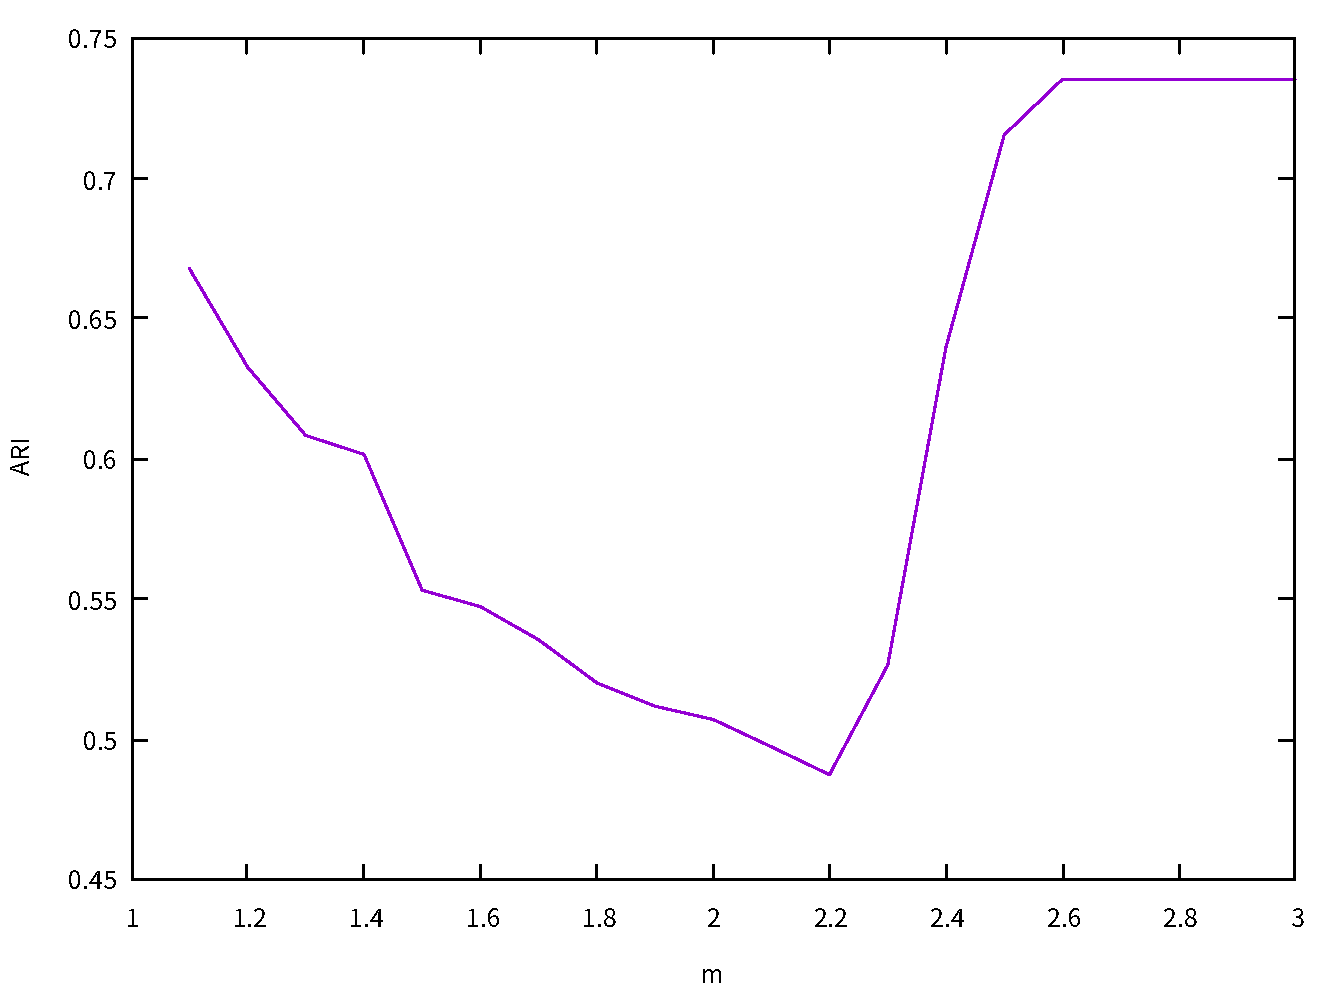
\includegraphics[width=\linewidth]{sFCMA_ARI.pdf}
    \caption{sFCMAの実データの実験結果}
    \label{fig:sFCMA_ARI}
   \end{minipage}
   \begin{minipage}{0.43\hsize}
    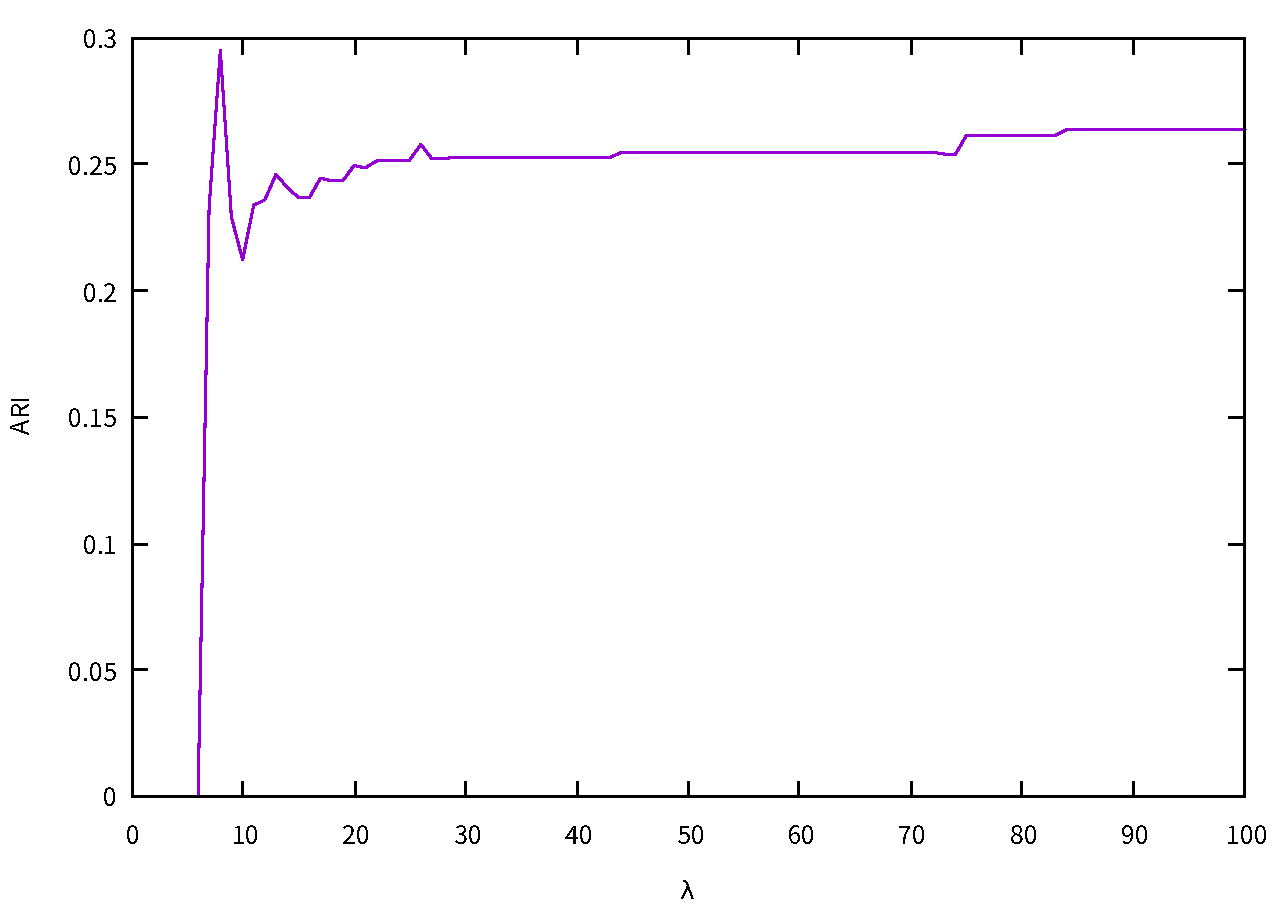
\includegraphics[width=\linewidth]{eFCMA_ARI.pdf}
    \caption{eFCMAの実データの実験結果}
    \label{fig:eFCMA_ARI}
   \end{minipage}
   \begin{minipage}{0.43\hsize}
    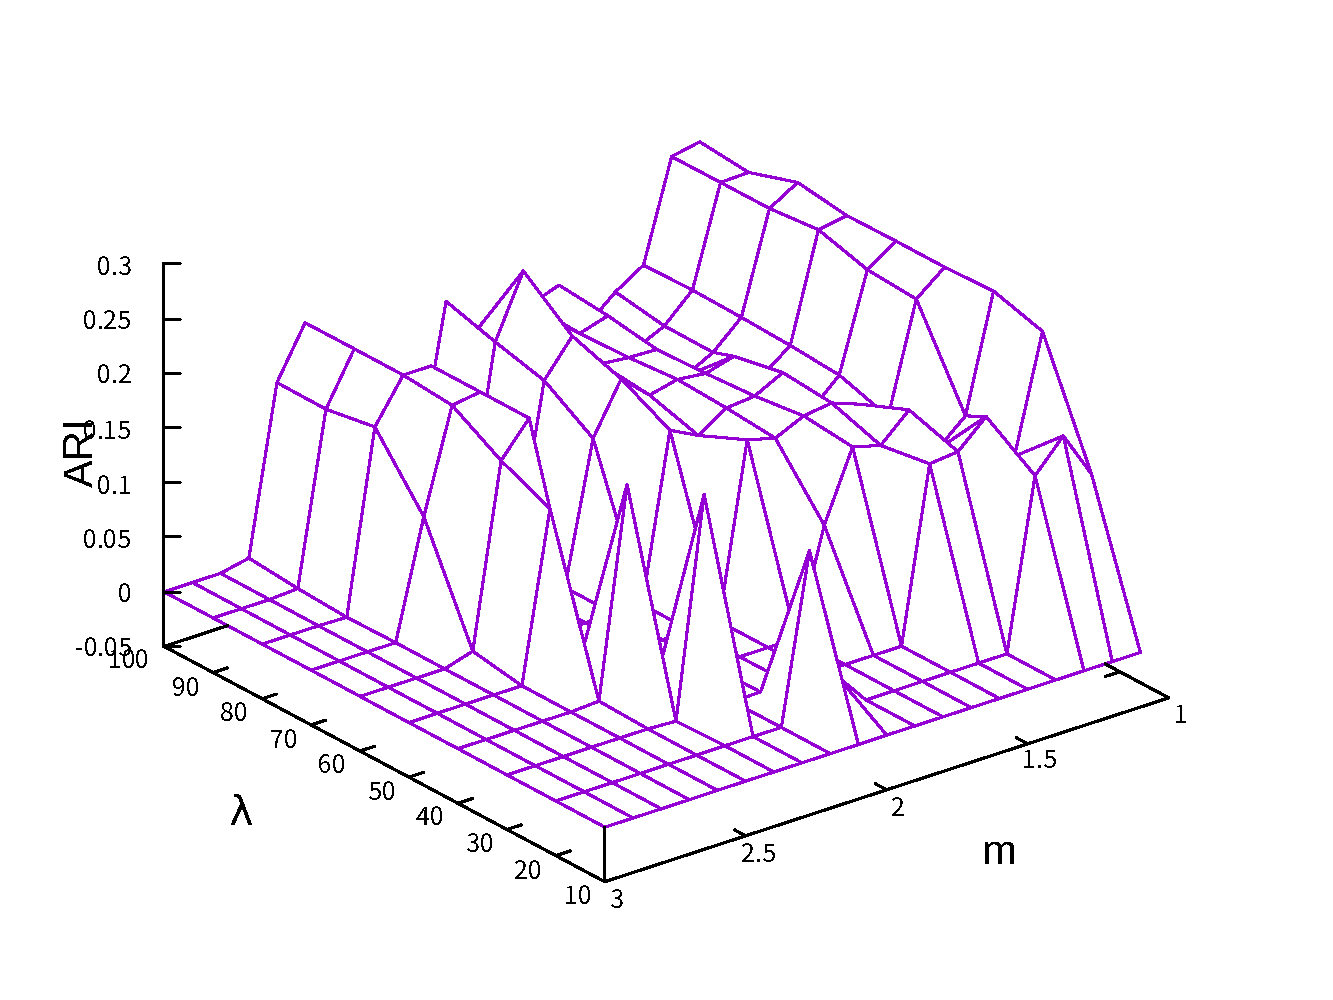
\includegraphics[width=\linewidth]{qFCMA_ARI.pdf}
    \caption{qFCMAの実データの実験結果}
    \label{fig:qFCMA_ARI}
   \end{minipage}
  \end{figure}

  \begin{table}[h]
   \centering
   \caption{各手法のARIの最高値とパラメータ}
   \begin{center}
    \begin{tabular}{ c || c | c }\hline
     手法名 & ARIの最高値 & パラメータ値\\ \hline \hline
     sFCMA & $0.73515$ & $m = 3$\\ \hline
     eFCMA & $0.29500$& $\lambda = 8$\\ \hline  
     qFCMA & $0.26286$ & $\lambda = 80$, $m = 1.1$\\  \hline
    \end{tabular}
    \label{tbl:max_ari}
   \end{center}
  \end{table}


  \section{おわりに}\label{sec:real_data_summary}
  本章では,実データを用いた実験について述べた.
  まず第\ref{sec:about_real_data}節で本実験で用いる人工データについて説明した.
  次に第~\ref{sec:real_data_algorythm}節でアルゴリズムについて述べた.
  最後に第\ref{sec:ari_compare}節で実験により得られた評価指標を用いて各手法の精度比較を行った.
  
  
\chapter{結論}\label{chap:conclusion}
本文書では,
第\ref{chap:suggest_method}章では,提案手法について説明した.
第\ref{chap:artificial_data}章では,人工データ実験により各手法の特性比較を行った.
第\ref{chap:real_data}章では,実データ実験により各手法の精度比較を行った.
最後に第\ref{chap:conclusion}章では,本文書の結論を述べた.
また,付録では,プログラムソースを掲載した.

本研究では,既に提案されていた3種のクラスタリング手法の特性と精度について現在に至るまで明らかになっていなかったため,
人工データを用いた特性比較及び実データを用いた精度比較を行った.
その結果として,
sFCMAは$m$が大きくなるとファジィになり,
eFCMAは$\lambda$が大きくなるほどクリスプになることが分かった.
また,qFCMAはsFCMAとeFCMAの両方の特性を併せ持つということが分かった.
精度はsFCMAが最も高評価となった.要因として,この手法の最適化問題にエントロピー項が含まれないということが考えられる.sFCMAの精度には,エントロピー項が含まれるeFCMA, qFCMAの2手法と比較して大きな差が見られた.
今後の課題は,今回用いなかった他の実データで$3$手法の比較を行い,精度についての裏付けを行うことである.

%
%
%
%
%
%
%\chapter{フォントのテスト}
%%
%%
%%
%\section{pifont}
%%
%%
%%
%\ding{"2E}\ding{"21}\Pisymbol{psy}{"A9}
%%
%%
%%
%\section{tascmac}
%%
%%
%%
%\keytop{A}\Return
%%
%%
%%
\begin{thebibliography}{5}
 \bibitem{sFCMA}Miyamoto, S., Kurosawa, N.: ``Controlling Cluster Volume Sizes in Fuzzy c-means Clustering'', Proc.~SCIS\&ISIS2004, pp.~1--4, (2004).
 \bibitem{eFCMA}Ichihashi, H., Honda, K., Tani, N.: ``Gaussian Mixture PDF Approximation and Fuzzy c-means Clustering with Entropy Regularization'', Proc.~4th Asian Fuzzy System Symposium, pp.~217--221, (2000).
 \bibitem{qFCMA}Miyamoto, S., Ichihashi, H., and Honda, K.: Algorithms for Fuzzy Clustering, Springer (2008).
 \bibitem{cFunc}宮本 定明, 馬屋原 一孝, 向殿 政男:``ファジイ $c$-平均法とエントロピー正則化法におけるファジィ分類関数'', 日本ファジィ学会誌 Vol.~10, No.~3  pp.~548--557, (1998).
 \bibitem{ARI} Hubert, L., and Arabie, P.:``Comparing Partitions'', Journal of Classifcation, Vol.~2, No.~1,
         pp.~193--218, (1985).
\end{thebibliography}
%
% \chapter*{感想}
% \addcontentsline{toc}{chapter}{感想}\label{chap:feel}
% おいしかった.
% \chapter*{謝辞}
% \addcontentsline{toc}{chapter}{謝辞}\label{chap:ack}
% ありがとう.
\appendix
\pagestyle{headings}
\addtocontents{toc}{\protect\diamondeleaders\par}
\chapter{プログラムソース}\label{chap:program}
 \section*{\texttt{vector.h}}
 \addcontentsline{toc}{section}{\texttt{vector.h}}
 \listinginput{1}{src/vector.h}
 \section*{\texttt{vector.cxx}}
 \addcontentsline{toc}{section}{\texttt{vector.cxx}}
 \listinginput{1}{src/vector.cxx}
 \section*{\texttt{matrix.h}}
 \addcontentsline{toc}{section}{\texttt{matrix.h}}
 \listinginput{1}{src/matrix.h}
 \section*{\texttt{matrix.cxx}}
 \addcontentsline{toc}{section}{\texttt{matrix.cxx}}
 \listinginput{1}{src/matrix.cxx}
 \section*{\texttt{randGaussianMain.cxx}}
 \addcontentsline{toc}{section}{\texttt{randGaussianMain.cxx}}
 \listinginput{1}{src/randGaussianMain.cxx}
 \section*{\texttt{hcm.cxx}}
 \addcontentsline{toc}{section}{\texttt{hcm.cxx}}
 \listinginput{1}{src/hcm.cxx}
 \section*{\texttt{hcm.h}}
 \addcontentsline{toc}{section}{\texttt{hcm.h}}
 \listinginput{1}{src/hcm.h}
 \section*{\texttt{sfcm.h}}
 \addcontentsline{toc}{section}{\texttt{sfcm.h}}
 \listinginput{1}{src/sfcm.h}
 \section*{\texttt{sfcm.cxx}}
 \addcontentsline{toc}{section}{\texttt{sfcm.cxx}}
 \listinginput{1}{src/sfcm.cxx}
 \section*{\texttt{efcm.h}}
 \addcontentsline{toc}{section}{\texttt{efcm.h}}
 \listinginput{1}{src/efcm.h}
 \section*{\texttt{efcm.cxx}}
 \addcontentsline{toc}{section}{\texttt{efcm.cxx}}
 \listinginput{1}{src/efcm.cxx}
 \section*{\texttt{qfcm.h}}
 \addcontentsline{toc}{section}{\texttt{qfcm.h}}
 \listinginput{1}{src/qfcm.h}
 \section*{\texttt{qfcm.cxx}}
 \addcontentsline{toc}{section}{\texttt{qfcm.cxx}}
 \listinginput{1}{src/qfcm.cxx}
 \section*{\texttt{sfcma.h}}
 \addcontentsline{toc}{section}{\texttt{sfcma.h}}
 \listinginput{1}{src/sfcma.h}
 \section*{\texttt{sfcma.cxx}}
 \addcontentsline{toc}{section}{\texttt{sfcma.cxx}}
 \listinginput{1}{src/sfcma.cxx}
 \section*{\texttt{efcma.h}}
 \addcontentsline{toc}{section}{\texttt{efcma.h}}
 \listinginput{1}{src/efcma.h}
 \section*{\texttt{efcma.cxx}}
 \addcontentsline{toc}{section}{\texttt{efcma.cxx}}
 \listinginput{1}{src/efcma.cxx}
 \section*{\texttt{qfcma.h}}
 \addcontentsline{toc}{section}{\texttt{qfcma.h}}
 \listinginput{1}{src/qfcma.h}
 \section*{\texttt{qfcma.cxx}}
 \addcontentsline{toc}{section}{\texttt{qfcma.cxx}}
 \listinginput{1}{src/qfcma.cxx}
 \section*{\texttt{sfcma\symbol{95}main\symbol{95}2d-Gaussian-2clusters.cxx}}
 \addcontentsline{toc}{section}{\texttt{sfcma\symbol{95}main\symbol{95}2d-Gaussian-2clusters.cxx}}
 \listinginput{1}{src/sfcma_main_2d-Gaussian-2clusters.cxx}
 \section*{\texttt{efcma\symbol{95}main\symbol{95}2d-Gaussian-2clusters.cxx}}
 \addcontentsline{toc}{section}{\texttt{efcma\symbol{95}main\symbol{95}2d-Gaussian-2clusters.cxx}}
 \listinginput{1}{src/efcma_main_2d-Gaussian-2clusters.cxx}
 \section*{\texttt{qfcma\symbol{95}main\symbol{95}2d-Gaussian-2clusters.cxx}}
 \addcontentsline{toc}{section}{\texttt{qfcma\symbol{95}main\symbol{95}2d-Gaussian-2clusters.cxx}}
 \listinginput{1}{src/qfcma_main_2d-Gaussian-2clusters.cxx}
 \section*{\texttt{sfcma\symbol{95}main\symbol{95}user-knowledge.cxx}}
 \addcontentsline{toc}{section}{\texttt{sfcma\symbol{95}main\symbol{95}user-knowledge.cxx}}
 \listinginput{1}{src/sfcma_main_user-knowledge.cxx}
 \section*{\texttt{efcma\symbol{95}main\symbol{95}user-knowledge.cxx}}
 \addcontentsline{toc}{section}{\texttt{efcma\symbol{95}main\symbol{95}user-knowledge.cxx}}
 \listinginput{1}{src/efcma_main_user-knowledge.cxx}
 \section*{\texttt{qfcma\symbol{95}main\symbol{95}user-knowledge.cxx}}
 \addcontentsline{toc}{section}{\texttt{qfcma\symbol{95}main\symbol{95}user-knowledge.cxx}}
 \listinginput{1}{src/qfcma_main_user-knowledge.cxx}

\end{document}

